%\documentclass[letterpaper, 12pt, parskip=full,DIV=10]{scrartcl}
% The next three lines are temporary, for todo notes, remove after notes are removed
\documentclass[letterpaper, 12pt, parskip=full,]{scrartcl}
\setlength{\marginparwidth}{4.5cm}
\usepackage[top=2.5cm, bottom=2.5cm, left=1.5cm, right=5cm]{geometry}
% Title and Subtitle added in .tex file
\usepackage{placeins} % for FloatBarrier to keep figures in right section
\title{Optimal Policies to Battle the Coronavirus ``Infodemic'' Among Social Media Users in Sub-Saharan Africa}
\subtitle{Preanalysis plan}
\author{Molly Offer-Westort, Leah R. Rosenzweig, Susan Athey}
\date{\today}

% USE: %\documentclass[letterpaper, 12pt, parskip=full,]{scrartcl}

\RequirePackage{etex}

% Graphics
\RequirePackage{graphicx}
\RequirePackage{epsfig}
\RequirePackage{psfrag}
\RequirePackage{wrapfig}
\RequirePackage[all]{xy}
\RequirePackage{listings}
\RequirePackage{verbatim} 
\RequirePackage{color} 
% Bold the 'Figure #' in the caption and separate it from the title/caption with a period
% Captions will be left justified
\RequirePackage[aboveskip=1pt,labelfont=bf,labelsep=period,justification=raggedright,singlelinecheck=off]{caption}


% Tables
\RequirePackage{float}
\RequirePackage{rotating}
\RequirePackage{array}
%\RequirePackage{minipage}
\RequirePackage{booktabs,threeparttable}

% Author
\RequirePackage[blocks]{authblk}
\renewcommand\Affilfont{\small}
\setlength{\affilsep}{0em}

\lstset{breaklines=true,basicstyle=\footnotesize\ttfamily}

% Document formatting
%\RequirePackage{fullpage}
\RequirePackage{setspace}
\RequirePackage{mathptmx}
\RequirePackage[hyphens]{url}
\RequirePackage{microtype} 
\RequirePackage[utf8x]{inputenc}
\RequirePackage{enumitem}
\setlist[itemize]{noitemsep, topsep=0pt}
\RequirePackage[colorinlistoftodos, textsize=footnotesize, color=blue!20!white]{todonotes} % adding to-do notes in working file
%\addtokomafont{disposition}{\normalfont\bfseries} % article fonts
%\setkomafont{descriptionlabel}{\normalfont\bfseries} % article fonts

% Bibliography and citation formatting
\RequirePackage[colorlinks=true, citecolor=blue]{hyperref}

\RequirePackage{nameref}
\RequirePackage[round]{natbib} 
\bibliographystyle{chicago}

% Title and Subtitle added in .tex file
%\author{Molly Offer-Westort}
%\date{\today}

\makeatletter %Set \Title reference
\let\Title\@title
\makeatother

\makeatletter %Set \Subtitle reference
\let\Subtitle\@subtitle
\makeatother

\makeatletter %Set \Author reference
\let\Author\@author
\makeatother

% Header and Footer
\RequirePackage{scrlayer-scrpage}
%\ihead{\textbf{\Title} }
%\ohead{\Author}

\RequirePackage{lastpage}
%\cfoot[]{}
%\ofoot[]{\thepage\ of \pageref{LastPage}}
\pagestyle{scrheadings}
%\setkomafont{pageheadfoot}{\small}
\RequirePackage{footnote}
\deffootnote[1.5em]{.5em}{1em}{\textsuperscript{\thefootnotemark}}


% Equation formatting
\RequirePackage{amsmath,amssymb,amsfonts} 
\RequirePackage{amsthm}
\RequirePackage{bbm}
\RequirePackage{array}
\newcommand\numberthis{\addtocounter{equation}{1}\tag{\theequation}}

\newtheorem{theorem}{Theorem}[section]
\newtheorem{lemma}{Lemma}[section]
\newtheorem{prop}{Proposition}[section]
\newtheorem{corollary}{Corollary}[section]
\newtheorem{hypothesis}{Hypothesis}


% Shortcuts
\newcommand{\nn}{\nonumber}

% Define new characters
\def\Var{{\textrm{Var}}\,}
\def\V{{\textrm V}\,}
\def\E{{\textrm E}\,}
\def\arg{{\textrm {arg} }\,}
\def\Cov{{\textrm{Cov} }\,}
\def\Cor{{\textrm{Cor} }\,}
\def\N{{\textrm N}\,}
\def\Supp{{\textrm {Supp} }\,}
\DeclareMathOperator*{\argmin}{arg\,min}
\DeclareMathOperator*{\argmax}{arg\,max}

%--------------------------------------------------------------------------
% Math boldface shortcuts, etc. ----------------------------------
%--------------------------------------------------------------------------
\newcommand{\A}{\mathbf{A}}\newcommand{\B}{\mathbf{B}}\newcommand{\C}{\mathbf{C}}
\newcommand{\D}{\mathbf{D}}\newcommand{\F}{\mathbf{F}}\newcommand{\G}{\mathbf{G}}
\newcommand{\HB}{\mathbf{H}}\newcommand{\I}{\mathbf{I}}\newcommand{\J}{\mathbf{J}}
\newcommand{\K}{\mathbf{K}}\newcommand{\Lb}{\mathbf{L}}\newcommand{\M}{\mathbf{M}}
\newcommand{\NB}{\mathbf{N}}\newcommand{\OB}{\mathbf{O}}\newcommand{\PB}{\mathbf{P}}
\newcommand{\Q}{\mathbf{Q}}\newcommand{\R}{\mathbf{R}}\newcommand{\SB}{\mathbf{S}}
\newcommand{\T}{\mathbf{T}}\newcommand{\U}{\mathbf{U}}%\newcommand{\V}{\mathbf{V}}
\newcommand{\W}{\mathbf{W}}\newcommand{\X}{\mathbf{X}}\newcommand{\Y}{\mathbf{Y}}
\newcommand{\Z}{\mathbf{Z}}

\newcommand{\aB}{\mathbf{a}}\newcommand{\bB}{\mathbf{b}}\newcommand{\cB}{\mathbf{c}}
\newcommand{\dB}{\mathbf{d}}\newcommand{\e}{\mathbf{e}}\newcommand{\f}{\mathbf{f}}
\newcommand{\g}{\mathbf{g}}\newcommand{\h}{\mathbf{h}}\newcommand{\iB}{\mathbf{i}}
\newcommand{\jB}{\mathbf{j}}\newcommand{\kB}{\mathbf{k}}\newcommand{\lB}{\mathbf{l}}
\newcommand{\m}{\mathbf{m}}\newcommand{\n}{\mathbf{n}}\newcommand{\oB}{\mathbf{o}}
\newcommand{\p}{\mathbf{p}}\newcommand{\q}{\mathbf{q}}\newcommand{\rB}{\mathbf{r}}
\newcommand{\s}{\mathbf{s}}\newcommand{\tB}{\mathbf{t}}\newcommand{\uB}{\mathbf{u}}
\newcommand{\vB}{\mathbf{v}}\newcommand{\w}{\mathbf{w}}\newcommand{\x}{\mathbf{x}}
\newcommand{\y}{\mathbf{y}}\newcommand{\z}{\mathbf{z}}

\def\AA{{\mathbb A}}\def\BB{{\mathbb B}}\def\CC{{\mathbb C}}
\def\DD{{\mathbb D}}\def\EE{{\mathbb E}}\def\FF{{\mathbb F}}
\def\GG{{\mathbb G}}\def\HH{{\mathbb H}}\def\II{{\mathbb I}}
\def\JJ{{\mathbb J}}\def\KK{{\mathbb K}}\def\LL{{\mathbb L}}
\def\MM{{\mathbb M}}\def\NN{{\mathbb N}}\def\OO{{\mathbb O}}
\def\PP{{\mathbb P}}\def\QQ{{\mathbb Q}}\def\RR{{\mathbb R}}
\def\SS{{\mathbb S}}\def\TT{{\mathbb T}}\def\UU{{\mathbb U}}
\def\VV{{\mathbb V}}\def\WW{{\mathbb W}}\def\XX{{\mathbb X}}
\def\YY{{\mathbb Y}}\def\ZZ{{\mathbb Z}}

\RequirePackage{euscript}
\let\muchmore= \gg
\let\muchless= \ll
\let\typewriter=\tt  % for turning on the typewriter font
\def\aa{{\EuScript A}}\def\bb{{\EuScript B}}\def\cc{{\EuScript C}}\def\dd{{\EuScript D}}
\def\ee{{\EuScript E}}\def\ff{{\EuScript F}}\def\gg{{\EuScript G}}\def\hh{{\EuScript H}}
\def\ii{{\EuScript I}}\def\jj{{\EuScript J}}\def\kk{{\EuScript K}}\def\ll{{\EuScript L}}
\def\mm{{\EuScript M}}\def\nn{{\EuScript N}}\def\oo{{\EuScript O}}\def\pp{{\EuScript P}}
\def\qq{{\EuScript Q}}\def\rr{{\EuScript R}}\def\ss{{\EuScript S}}\def\tt{{\EuScript T}}
\def\uu{{\EuScript U}}\def\vv{{\EuScript V}}\def\ww{{\EuScript W}}\def\xx{{\EuScript X}}
\def\yy{{\EuScript Y}}\def\zz{{\EuScript Z}}

\newcommand{\Beta}{\boldsymbol{\beta}}
\newcommand{\btheta}{\boldsymbol{\theta}}
\newcommand{\bgamma}{\boldsymbol{\gamma}}
\newcommand{\bpi}{\boldsymbol{\pi}}
\newcommand{\arrowp}{\stackrel{p}{\rightarrow}}
\newcommand{\0}{\mathbf{0}}
\newcommand{\bP}{\mathbf{P}}

\newcommand\independent{\protect\mathpalette{\protect\independenT}{\perp}}
\def\independenT#1#2{\mathrel{\rlap{$#1#2$}\mkern2mu{#1#2}}}


\newcommand{\indep}{\perp\!\!\!\!\perp}

\thispagestyle{plain}



\begin{document}%
\normalsize%
\maketitle%
\tableofcontents%
\clearpage%


\centerline{\textbf{ABSTRACT}}
\begin{abstract}
Alongside the outbreak of the new coronavirus, much of the world’s population is also experiencing an “infodemic” -- the spread of myths and hoax cures related to the virus through online media outlets and social media platforms. While many false cures are largely harmless (e.g., drinking lemon water), others have potentially devastating consequences, such as misuse of chloroquine. As a result, governments struggling to prepare healthcare systems and encourage citizens to comply with best practices also need to tackle misinformation. Building upon the experimental literature on combating fake news, we evaluate the effect of interventions designed to decrease sharing of false COVID-19 cures. Using Facebook advertisements to recruit social media users in Kenya and Nigeria, we deliver our interventions using a Facebook Messenger chatbot, allowing us to observe treatment effects in a realistic setting. Using a contextual adaptive experimental design to sequentially assign treatment probabilities, we are able to learn the optimal contextual policy, and minimize assignment to ineffective or counter-productive interventions within the experiment. Analyzing heterogeneity in treatment effects allows us to learn whether different interventions are more effective for different people, improving our understanding of how to tackle harmful misinformation during an ongoing health crisis. Finally, we bring comparative data to a global problem for which the existing research has largely been limited to the U.S. and Europe. This pre-analysis plan describes the research design and outlines the key hypotheses that we will evaluate.
\end{abstract}





\section{Motivation and Research Questions}

% motivation
Alongside the outbreak of the novel coronavirus (SARS-CoV-2), much of the world's population is also experiencing an ``infodemic'' -- the spread of myths and hoax cures related to the virus. COVID-19 misinformation has been spreading through online media outlets and social media platforms. Falsities and conspiracy theories cover topics from government activities to scam opportunities for aid and hoax cures. In some places citizens remain in disbelief and denial of the very existence of the virus.\footnote{\url{https://www.bbc.com/news/world-africa-53403818}} 

Though challenging to calculate the $R_0$ of these falsities, evidence suggests that the spread of hoax cures can be particularly deadly. Purported cures for COVID-19 that have circulated on social media include both benign recommendations such as drinking lemon water and inhaling steam, but also include others that can have devastating consequences if adopted, such as misusing chloroquine or drinking bleach. In Iran, dozens of people died from alcohol poisoning after ingesting methanol to stave off the coronavirus.\footnote{\href{https://nationalpost.com/news/world/rumours-that-alcohol-kills-covid-19-leaves-21-iranians-dead-from-poisoning}{Bloomberg News}, Mar. 10, 2020.} In Nigeria, multiple people were hospitalized for chloroquine poisoning following statements by president Trump suggesting the medication could be used to treat COVID-19. \footnote{\href{https://www.cnn.com/2020/03/23/africa/chloroquine-trump-nigeria-intl/index.html}{CNN}, Mar. 23, 2020.} If the spread of COVID-related information follows the trajectory of other types of online information, we might expect false information to spread more than true information \citep{vosoughi2018spread}. Though identifying the causal link between online rumors and offline behaviors is challenging, activity on social media and the internet more generally has been linked to offline behaviors such as hate crimes \citep{muller2019fanning, chan2016internet}. As a result, governments struggling to prepare health care systems and encourage citizens to comply with best practices are also struggling to tackle a pandemic of online misinformation.

% what we do 
This project evaluates the effect of interventions designed to decrease sharing of false COVID-19 cures. Using Facebook advertisements to recruit social media users in Kenya and Nigeria, we deliver our interventions using a Facebook Messenger chatbot, allowing us to observe treatment effects in a realistic setting and environment where such stories have appeared. Other studies have demonstrated that sharing behavior in online surveys mirror those of real-world social media users \citep(mosleh2020self). We test interventions targeted at both the respondent level, such as tips for spotting fake news, a video training and nudges, as well as headline-level treatments, such as ``false'' tags and related articles. All of the treatments are described in Table~\ref{tab:treatments}. 

Using a contextual adaptive experimental design, we sequentially assign treatment probabilities to privilege assignment to the most effective interventions, and minimize assignment to ineffective or counter-productive interventions. Our aim is to learn an optimal contextual policy that will assign respondents the intervention that is most effective for them, conditional on their covariate profile. Exploring heterogeneity in treatment effects allows us to learn whether different interventions are more effective for different people, improving our understanding of how to tackle harmful misinformation during an ongoing health crisis. 

% how we build on existing lit
This work builds on the experimental literature on combating fake news in several important ways. First, we examine several prominent interventions that have proven successful in other studies and in other settings using an adaptive design to observe the best intervention policy. Second, we bring comparative data to a global problem. Despite the global nature of the ``infodemic,'' much of the existing research has been focused on the Global North, particularly the United States \citep{pennycook2020fighting, bursztyn2020misinformation}.\footnote{Two recent exceptions from sub-Saharan Africa include a field experiment in Zimbabwe using Whatsapp messages from a trusted NGO  to counter COVID misinformation \citep{bowles2020center} and a recent survey among traders in Lagos, Nigeria looking at the correlates of belief in COVID-related misinformation \citep{Grossman2020}.} This pre-analysis plan describes the research design, outlines the key hypotheses that we will evaluate, and details our approach to analysis.




\section{Case Selection and Stimuli}
% Why kenya + Nigeria?

We examine these questions using a study focused on online social media users in two major English-language hubs of online communication in sub-Saharan Africa, Kenya and Nigeria.  Collectively, Facebook estimates there are 30-35 million Facebook users who are 18 years and older from these two countries (as reported on \href{https://www.facebook.com/business/insights/tools/audience-insights?ref=ens_rdr}{Facebook's advertising platform}). Misinformation and fake news are major problems in these countries. AfricaCheck.org, a third party verification site, has offices in both countries and has recently created pages devoted to coronavirus-related misinformation circulating online. From January to March, the number of English-language fact-checks increased by more than 900\% worldwide \citep{brennen2020types}, demonstrating the prevalence of this kind of content and the availability of verified coronavirus-related information.  Figure \ref{fig:poynter} illustrates the volume of fact checks that appear in \url{poynter.org}'s global coronavirus facts database, which demonstrates that Kenya and Nigeria are main factcheck sources on the continent. Thus, there is a large database of verified information from which we can draw stimuli for our experiment in these two countries. 

\begin{figure}[!htb]
\centering
\caption{Map illustrating the volume of fact-checks in \url{poynter.org}'s global coronavirus facts database.}
\label{fig:poynter}
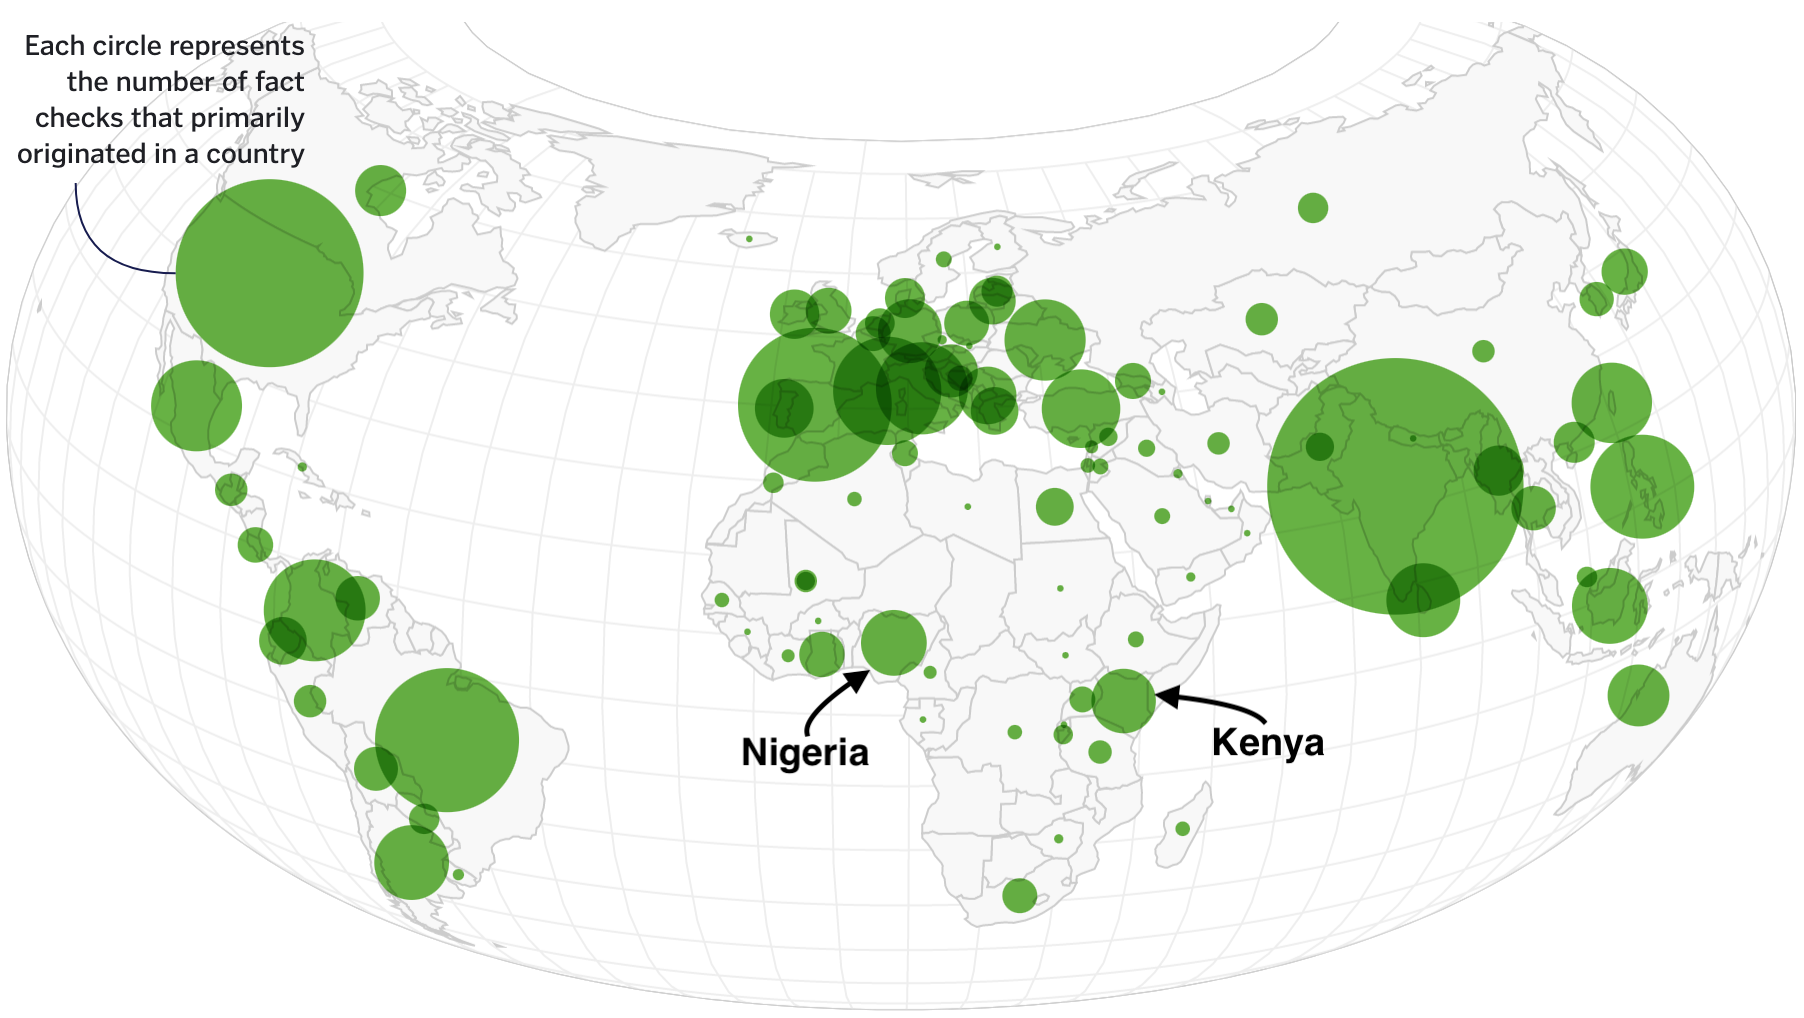
\includegraphics[width=.95\textwidth]{poynter2.png}
\end{figure}

For this experiment, we focus on COVID-19 prevention and cure-related information because this comprises a large proportion of the overall coronavirus-related information that has been fact-checked by experts (see Figure \ref{fig:poynter_cures}) and also serves as some of the most dangerous misinformation. Some hoax cures, when adopted, can be deadly. Moreover, even if not adopted when claims about the existence of a cure circulate widely they may deter people from taking preventative measures. We acknowledge that interventions will likely need to be specific to the particular type of misinformation being targeted, whether political, health-related, etc. The focus of this paper is on prevention and cure-related (mis)information that is immediately relevant for the ongoing pandemic. 
%\todo{Should this be moved to a new 3.3.2 Stimuli section?} - kept here and changed section heading

To collect stimuli we adopted several criteria to search for both false and true pieces of information related to coronavirus prevention techniques and COVID-19 cures. First, we searched AFP, Poynter, and AfricaCheck website for any of this type of misinformation that had been checked by these organizations that appeared online in Kenya and Nigeria since the start of the pandemic in early March 2020. Second, we collected WHO myth-buster infographics that directly countered the misinformation items we found. We also collected prevention messaging from the Nigeria Center for Disease Control, National Emergency Response Committee in Kenya, and the Ministry of Health in both countries, as these are the main government entities combating the spread of the disease in these countries and official sources of information. Our full set of stimuli for each country is presented in Appendix~\ref{appendis:stimuli}. 

%% LR: I'm looking for citations to demonstrate these are hubs of misinfo - another way to go is that they are major english media sources and other countries in the region often also read news from ky/ng...




\begin{figure}[t]
\centering
\caption{Map illustrating the volume of COVID-19 cure-related fact-checks in \url{poynter.org}'s global coronavirus database.}
\label{fig:poynter_cures}
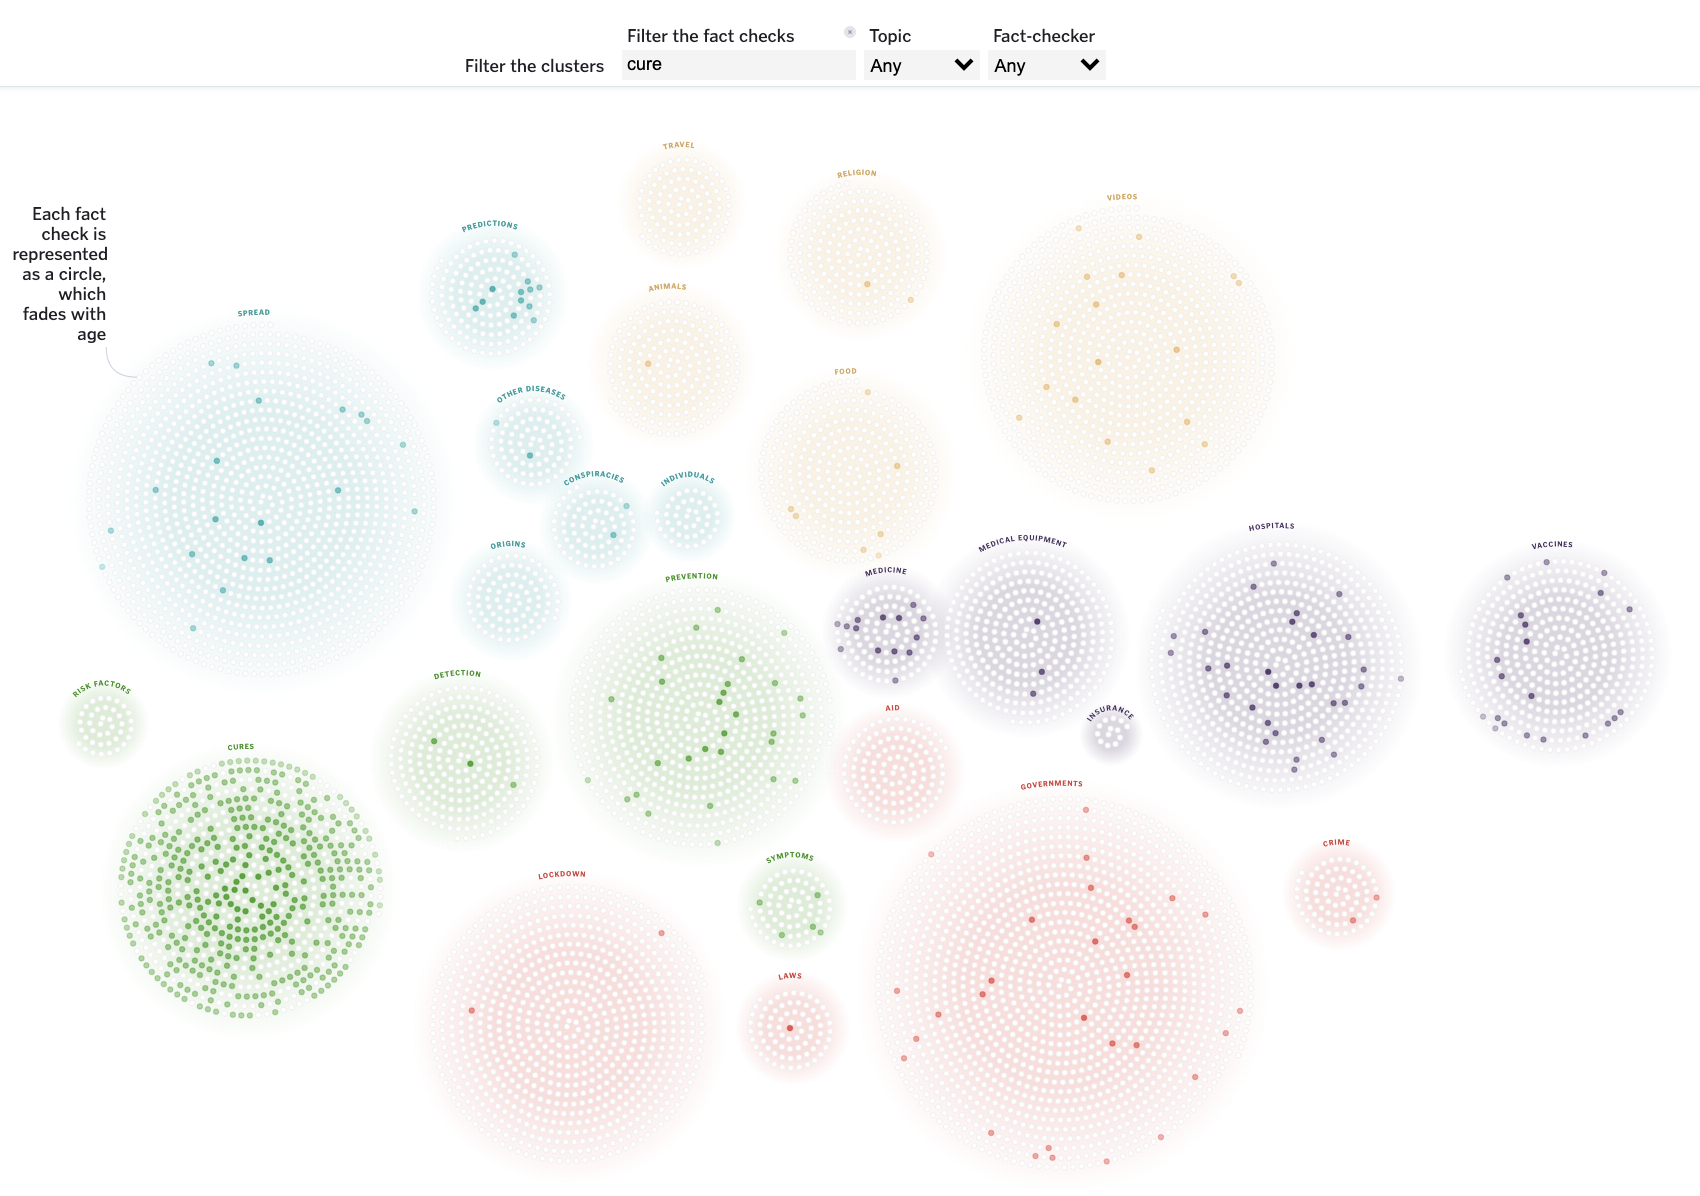
\includegraphics[width=.95\textwidth]{poynter_cures.png} 
\end{figure}
% https://www.poynter.org/coronavirusfactsalliance/


\FloatBarrier
\section{Experimental Setup}



\subsection{Sample recruitment}
We will recruit respondents in Kenya and Nigeria using Facebook advertisements targeted to users 18 years and older living in these countries.\footnote{Based on previous work it is clear that Facebook imputes location information for some of its users, which can be inaccurate. We will also ask a location screening question to ensure our respondents live in our countries of interest.} %
To achieve balance on gender within our sample we create separate ads targeting men and women in both countries. Our target sample size is 1,500 respondents in each country for our pilot. Size of the full scale study will be determined following piloting, in procedures described in Section~\ref{simulations}.


Advertisements will appear within Facebook or Instagram, offering users with the opportunity to ``Take a 20 minute academic survey on Messenger - receive airtime.'' Incentives will be approximately 0.50-0.55 USD, accounting for transaction and messaging fees on the \href{https://africastalking.com/}{Africa's Talking} airtime distribution platform.%
\footnote{The recruitment advertisement is shown in Figure~\ref{fig:ad} in Appendix~\ref{appendix:recruitment}.} %
 When users click on the ``Send Message'' button on our advertisement, a Messenger conversation will open with our Facebook page, starting a conversation with a chatbot programmed to implement the survey.%
 \footnote{\color{red}{[[TK: images of chatbot once linked to page]]}} % 
 In contrast to sending users to an external survey platform such as Qualtrics, the benefit of the chatbot is that we keep users on the Facebook platform, with which they are likely more familiar, and maintain a realistic setting in which users might encounter online misinformation.  Respondents who complete the survey in the chatbot will receive compensation in the form of mobile phone airtime sent to their phone. %%MOW: confirm survey completion time--and update advertisement accordingly


\subsection{Covariates}
Through the chatbot, we collect demographic and other information on respondents.  We use the below covariates for learning conditional treatment assignment probabilities in the chatbot. The full list of covariates and question wording is in Appendix~\ref{appendix:covariates}. %\todo{Full approach to implementation of treatment assignment probabilities in progress. } %% LR: commented out for now...

\input{covariates_shortform.tex}

For missing covariate information, we will follow the procedures in \cite{greensop1.05}: for a given covariate, if no more than 10 percent of total covariate values are missing, recode missing values to the overall mean; if greater than 10 percent of covariate values are missing, introduce a missingness flag. 

\subsection{Treatment}
Drawing on the literature on experimental interventions to combat misinformation, we include several interventions designed to reduce the spread of misinformation online, which are targeted both at the respondent level and headline level. This list of treatments also draws on real-world interventions that companies and platforms have instituted to combat misinformation. Treatments are presented in Table~\ref{tab:treatments}. 

% interesting point to maybe incorporate: Facebook, 24% of false-rated content in our sample remains up without warning labels \citep{brennen2020types}

\begin{table}[H]
\begin{tabular}{l|l|l}
\multicolumn{1}{c|}{\textbf{\begin{tabular}[c]{@{}c@{}}Shorthand\\ Name\end{tabular}}} & \multicolumn{1}{c|}{\textbf{\begin{tabular}[c]{@{}c@{}}Treatment\\ Level\end{tabular}}} & \textbf{Treatment}                                                                                                                                                                                                                                                                                                                                                                                              \\ \hline
Facebook tips                                                                                                           & Respondent                                                                                                   &  Facebook's ``Tips to Spot False News'' 
\\
AfricaCheck tips                                                                                                         & Respondent                                                                                                   &  \url{Africacheck.org}'s guide: \\ & & ``How to vet information during a pandemic''                                                                                                                                                                                                                                                                                                                             \\
Video training                                                                                                     & Respondent                                                                                                   &  \href{https://www.bbc.com/news/av/embed/p088bh96/52118949}{BBC Video training}                                                                                                                                                                                                                                                                                                                                                                                  \\
Emotion suppression                                                                                                       & Respondent                                                                                                   & \begin{tabular}[t]{@{}l@{}}Prompt: ``As you view and read the headlines, if you have any \\feelings, please try your best not to let those feelings show.  \\Read all of the headlines carefully, but try to behave so that \\someone watching you would not know that you are feeling\\ anything at all” \citep{gross1998emerging}.\end{tabular}
\\
Pledge                                                                                 & Respondent                                                                                                   &  \begin{tabular}[t]{@{}l@{}} Prompt: Respondents will be asked if they think misinformation \\ is a problem, if they're willing to help stop it, and finally if they're \\willing to take either a \textit{private} or \textit{public} pledge to stop the spread \\of false COVID-19 cures online (see exact text in \ref{sec:pledge}).
\end{tabular}
\\
Accuracy nudge                                                                                 & Respondent                                                                                                   & Placebo headline: ``To the best of your knowledge, is this headline \\& & accurate?'' \citep{pennycook2020fighting, pennycook_epstein_mosleh_arechar_eckles_rand_2019}.
\\
Deliberation nudge                                                                                 & Respondent                                                                                                   & Placebo headline: ``In a few words, please say \textit{why} you would\\ & & like to share or why you would not like to share this headline.''\\ & & [open text response]
\\
%Context                                                                                                        & Headline                                                                                                     & \begin{tabular}[t]{@{}l@{}}Facebook context button; if you click the info button on an\\ article, a pop-up tells you a few facts about the source: \\ how long the Facebook page has been registered,\\ and has a flag if article is more than 90 days old\end{tabular}
%\\
%Flag                                                                                                           & Headline                                                                                                     &  ``Disputed" flag on the headline                                                                                                                                                                                                                                                                                                                                                     \\
Related articles                                                                                                       & Headline                                                                                                     & Facebook-style related stories: below story,\\ & & show one other story which corrects a false news story                                                                                                                                                                                                                                                                                             \\
Factcheck                                                                                                      & Headline                                                                                                     & Fact checking flag from third party\\ & & (e.g., Facebook, AFP, AfricaCheck, etc)
 \\
More information                                                                                                      & Headline                                                                                                     & Provides a link to ``Get the facts about COVID-19''\\ & & as per Twitter flags
 \\
Control                                                                                                        & N/A                                                                                                          & Control condition                                                                                                                                                                                                                                                                                                                                                                                              
\end{tabular}
\caption{Description of interventions included in the experiment}
\label{tab:treatments}
\end{table}

Respondent-level treatments and headline-level treatments are implemented as separate factors, each of which has an empty baseline level that is the control. So respondents may be assigned the pure control condition, one of the respondent-level treatments but no headline-level treatment, one of the headline level treatments but no respondent-level treatment, or one of the respondent-level treatments \textit{and} one of the headline-level treatments. 


\subsection{Outcomes and Response Function}

We are interested in decreasing sharing of harmful false information about COVID-19 cures and treatments while not negatively impacting sharing of useful information about transmission and best practices from verified sources. Specifically, we are interested in three outcomes: (1) Self-reported intention to share a given story, (2) Actual behavior with respect to sharing that story\footnote{Though this is only measured for the \textit{true} headlines as respondents are mostly prevented from sharing the falsehoods.}, (3) Willingness to share tips and information about misinformation more generally. For all reported outcomes and responses (excluding aggregated tallies discussed below), analysis will be conducted as described in Section~\ref{analysis}.  

\subsubsection{Primary Response Function}

We measure interest in sharing information through two questions:
\begin{itemize}
\item Would you like to share this post on your timeline? 
\item Would you like to send this post to a friend on Messenger?
\end{itemize}

Prior to treatment, we show respondents two articles from their country randomly sourced from our misinformation stimuli and two articles randomly sourced from our true information stimuli, in random order, and for each stimuli we ask the above self-reported interest questions. Respondents are then asked a series of unrelated questions, and are then randomly assigned treatment according to the experimental design. If assigned one of the respondent-level treatments, they are administered the relevant treatment. They are then shown two additional misinformation stimuli and two additional true information stimuli, selected from the remaining stimuli that they were \textit{not} shown pre-treatment. If the respondent is assigned a headline-level treatment, this treatment is applied only to the misinformation stimuli, as flags and fact-checking labels are not generally applied to true information from verified sources.\footnote{The initial implementation of Twitter's labeling of coronavirus-related tweets with links to additional information was deemed to be overly broad, and was applied to some tweets that did not include misinformation. Twitter revised their labeling in late June of 2020. A company message was released here on June 26: \url{https://twitter.com/TwitterSupport/status/1276661483561029632}. } For each of the stimuli we again ask the same self-reported sharing intention questions. 

By using a pre-test / post-test design  \citep{davidian2005semiparametric} %https://declaredesign.org/library/articles/pretest_posttest.html
and an index of repeated measures \citep{broockman2017design}, we aim to improve the efficiency of our effect estimation. 


We code response to the self-reported interest questions as 1 if the respondent affirms and 0 otherwise. Let $M_i^1$ be the sum of respondent $i$'s pre-test responses to the \textit{misinformation} stimuli and let $T_i^1$ be the sum of respondent $i$'s pre-test responses to the \textit{true} informational stimuli. $M_i^2$ and $T_i^2$ are the respective post-treatment responses. Then $M_i^1, T_i^1, M_i^2, T_i^2 \in {0,1,2,3,4}$. 

Our pre-test outcome is then:
\[
Y^1_i = M_i^1 + 0.5 T_i^1,
%Y_i = -(M_i^2 - M_i^1) + 0.5 \times (T_i^2 - T_i^1)
\]%\todo{LR:Made me wonder whether we want to, for power sake, use random effects model w/respondent and headline level REs? so rather than using DV that sums shares across all 4 headlines seen ? This is how psych misinfo studies usually analyze headline-level outcomes and deal with respondent and headline correlations.\MOW: Let's discuss, I'm not sure what this would look like for our adaptive agent model. }
And the respective post-test response function is $Y^2_i$ with the relevant terms on the righthand side. In our approach to analysis, we will condition on $Y^1$ on the righthand side of the equation, keeping $Y^2$ on the lefthand side. For notational convenience, we will refer to $Y^2$ as $Y$ going forward. This response function will be the variable which we optimize for in our adaptive algorithm described in Section~\ref{adaptiveagent}, and in our policy learning described in Section~\ref{analysis}. Because of random assignment, we expect to see no systematic differences in pre-test interest in sharing either true or untrue stimuli across treatment conditions, conditional on covariates. %For a given treatment condition, all else equal, if respondents share misinformation at lower rates post-test compared to control, this will result in a relatively higher response variable. If respondents share true information at lower rates post-test compared to control, this will result in a relatively lower response variable, but the relative impacts are only half as large as those for the misinformation stimuli. 




\subsubsection{Secondary Outcomes}
Additionally, we measure secondary behavioral outcomes which allows us to further investigate the extent to which treatments may suppress the sharing of \textit{true} information.

In order to obtain a behavioral measure of sharing, we collect the articles the respondent indicated they would like to share throughout the survey and at the end of the survey provide links to the \textit{true} information. For these true stimuli, we offer respondents the opportunity to actually share this information as a Facebook post, which has been created on our project Facebook page. We are able to measure whether respondents click on a button which opens a pop-up screen to share the post on Facebook, however, we cannot measure directly whether they then actually follow through to the second step and post the article on their own timeline. Consequently, we report only rates of clicking the initial share button. The response function here is measured as the percent of true stimili that the respondent said they wanted to share during the survey for which they later click the button to share on Facebook. (We do not differentiate between stimuli presented pre- and post- treatment here, since the behavioral response measurement for all stimuli is all post-treatment.) To provide some insight on the extent to which respondents followed up on an intention to share, we report the \textit{aggregate} number of times the associated post for each stimuli was shared. %We \textit{could} actually create a separate post for each treatment combination, and measure sharing that way, but this seems like overkill for a secondary outcome in an already complicated project.

At this point we also debrief respondents, informing them about the headlines they were shown that are false. Instead of allowing respondents to share these headlines, we provide links to tips for spotting misinformation online and also offer them the opportunity to share these tips on their timeline or on messenger; we measure intention to share these tips and aggregate number of shares of tips by treatment condition as well. 


\subsubsection{Attrition} We will include in analysis all respondents for whom we have collected complete pre-test responses. As treatment is not revealed at this point, attrition should be independent of treatment assignment conditional on covariates. For respondents who attrit after collection of pre-test responses and before collection of post-test responses, all types of post-test responses will be coded as zero.\todo{Alternatively, could use \cite{davidian2005semiparametric} Robins/Rotnitzky/Zhao approach in final analysis.}


\section{Hypotheses and Data Collection}



Our data is described by treatments $W_i \in \ww$\footnote{Our treatments are composed of two separate factors, but here we use $W$ to represent combined treatment conditions. Where we wish to explicitly differentiate, we use $W^R_i$ and $W^H_i$ for respondent- and headline-level treatments respectively. As each factor includes a baseline level absent intervention, the cardinality $|\ww| = |\ww^H|\times |\ww^R|$.}; response,  $Y_i \in \RR$; and covariates, $X_i \in \xx$. 

We assume the data is indexed by $i = 1, \dots, N$ where indexing represents the order in which respondents entered the experiment; this allows us to use $i$ to also represent relative chronological relationships in our sequential adaptive design. 

We use potential outcome notation, where $Y_i(w)$ represents the potential outcome for respondent $i$ under treatment $w$, and by experimental design,  we have strong ignorability of potential outcomes to treatment conditional on observed covariates. 


We would like to learn and evaluate an optimal contextual policy, under which we assign the most effective treatment conditional on covariates. Formally, a policy maps a set of covariates to a decision \citep{athey2017efficient}, %\todo{Update reference}
\begin{align}
  \pi: \xx \rightarrow \ww. 
  \label{eq:policy}
\end{align}
In our setting, we will learn this policy, $\hat \pi$, and evaluate its value. The value of a policy is defined as, 
\begin{align}
V(\pi) =  \E[Y(\pi(X_{i}))],
  \label{eq:policy_value}
\end{align}
where the expectation is taken over the distribution of $X$.\footnote{Here we will only consider deterministic policies, but for a random policy, the expectation will be taken over the joint distribution. }

\subsection{Hypotheses}\label{hypotheses}

Our hypotheses of interest relate the value of an estimated optimal contextual policy $\pi_{opt}$ to fixed policies $\pi_{W}$, where under each fixed policy we would assign all respondents the relevant treatment $w$. The control policy is the fixed policy $\pi_{w_{C}}$

Our primary hypothesis is that we are able to estimate from the data an optimal contextual policy that improves over the control. 
  \begin{hypothesis}
  The best contextual policy that can be estimated from the data achieves higher value than the control treatment \label{eq:optctr}.
\begin{align}
  H_{0}: V(\pi_{opt}) = V(\pi_{w_{C}}) \qquad H_{a}:  V(\pi_{opt}) > V(\pi_{w_{C}})
\end{align}
\end{hypothesis}
This is the hypothesis that we aim to optimize for in our adaptive data collection. 

We would also like to learn how much we gain by exploiting heterogeneity in the data. As a secondary hypothesis, we propose that the optimal policy that we are able to estimate from the data improves over the best fixed policy. 
  \begin{hypothesis}
  The best contextual policy that can be estimated from the data achieves higher value than the best fixed policy, i.e., the fixed policy with the highest associated value. 
  \label{eq:optmax}
\begin{align}
  H_{0}: V(\pi_{opt}) = \argmax_w V(\pi_{w}) \qquad H_{a}:  V(\pi_{opt}) > \argmax_w V(\pi_{w})
\end{align}
\end{hypothesis}


\subsection{Adaptive data collection}\label{adaptiveagent}

To collect data with the objective of learning an optimal policy, we use a \textit{contextual bandit} algorithm, in which we sequentially update treatment assignment probabilities based on the observed history of treatments, response, and covariates. These types of algorithms navigate a tradeoff in \textit{exploration} of the treatment space with \textit{exploitation} of those treatments which we have observed to be effective based on historical data. This allows us to continue to learn about treatment effect heterogeneity while continuing to improve outcomes over time \textit{within} the frame of the experiment. 

We will use a version of linear Thompson sampling \citep{agrawal2013thompson}. Under Thompson sampling \citep{thompson1933likelihood,thompson1935theory}, treatment is assigned according to the Bayesian posterior probability that each treatment is best. In linear Thompson sampling, this is generalized to allow the outcome to be a linear function of covariates. We use a batched approach to updating, collecting data in batches and then updating treatment assignment model after each batch. 

This algorithm requires us to se a number of design parameters; the procedures to select these parameters are discussed below in Section~\ref{simulations}. 

% \label{subsec:exploration_methods}
Our implementation is based on the balanced linear Thompson sampling method described in \cite{dimakopoulou2017estimation, dimakopoulou2019balanced} :

\begin{enumerate}
\item In the first batch, $b = 1$, we assign treatment uniformly at random. \todo{The bootstrapping aspect of this algorithm is adapted from the Cameroon PAP. Check wording and ensure that appropriate attribution is given. }

\item For equally sized batches $b = 2, \dots, B-1$:

\begin{enumerate}
 \item Fit a ridge regression model. Compute the minimum mean cross-validated error value of the penalization factor $\lambda^{CV}$ using the entire observed history of data.\footnote{For the agent we use a linear model, with treatment indicators, covariates, and treatment and covariates interacted:
 
\begin{align*}
\hat{\mu}_w(X_{i}) & =
			\sum_{w^R} 1\{W^R_i = w^R\}\hat\beta_{w^R}  +
			\sum_{w^H} 1\{W^H_i = w^H\}\hat\beta_{w^H}  +\\ 
			& \sum_{w^R} \sum_{w^H}1\{W^R_i = w^R\} \times 1\{W^H_i =  \hat w^H\}\hat\beta_{w^{R,H}} +  \\
			& \sum_{\ell}  X_{[\ell]i}\hat{\beta}_{\ell} +\\
        &  \sum_{w,\ell} 1\{ W_{i} = w\} X_{[\ell]i} \hat{\beta}_{w, \ell}.\numberthis
         \label{eq:linear_model_full}
\end{align*} 
The model is estimated using $L_{2}$ penalties for regularization, exclusive of the main treatment effects $\beta_{w^R}$ and $\beta_{w^R}$. 
Observations are weighted according to rolling stabilized inverse probability weights using known assignment probabilities, following \cite{dimakopoulou2017estimation}. Stabilized inverse probability weights are discussed in Appendix~\ref{appendix:stabilized}. Recall that the pre-test response is implicitly included on the righthand side of the model. }
\todo{Alternative option: Have separate penalty factors, e.g., one for just covariates, one for interactions of treatment x treatment and treatment x covariates jointly. }
\todo{Comment for Vitor: does it even make sense to do batch-wise stabilized weights? Do we have recorded implementation in bandits or adaptive-inference repo?}

  \item \label{step:draw} Draw $M$ random samples with replacement from the data, with samples indexed by $m = 1, \dots, M$, so that data from sample $m$ is represented by $D^{(m)} := (X^{(m)}, W^{(m)}, Y^{(m)})$.\footnote{We set M = 100.} 

  \item Within each sample, for each possible context $x$\footnote{We note that for the adaptive agent, we only use the restricted covariate set described in Table~\ref{cov_short}. }, treatment $w$ and bootstrap sample, estimate conditional means  $\hat{\mu}_w^{(m)}(x)$ for each treatment using the fitted outcome model, where $\mu_w(x) = \E[Y(w)|X=x]$. The penalization value is fixed as $\lambda_{CV}$ from step 1, without performing any additional cross-validation.
  
  \item For each context $x$ and available treatment $w$, compute and store the following statistics representing the average value of each treatment, and the uncertainty associated with this statistic.
    \begin{equation}
      \begin{aligned}
        \hat{\mu}_w(x)         &= \frac{1}{M}\sum_{m} \hat{\mu}_w^{(m)}(x) \\
         \hat{\sigma}^{2}_w(x) &= \frac{1}{M(M-1)} \sum_{m} (\hat{\mu}_w^{(m)}(x) - \hat{\mu}_w(x))^2
      \end{aligned}
    \end{equation}

  \item \label{step:prob} Approximate the probability that each treatment $w$ is maximal for each possible context $x$. In order to do that, we draw from the following probability distribution a large number $S$ times\footnote{We set S = 1,000.}
  \begin{align}
    \theta_{w}(x) \sim \mathcal{N}(\hat{\mu}_w(x), \hat{\sigma}_w^{2}(x)) \qquad %\text{for } s \in \{1, \cdots, S\} \text{ and treatment }w
    \text{ for all treatments }w
  \end{align}

  and compute the fraction of times that treatment $w$ was the largest for each $s$ set of draws
  \begin{align}
    q_{b}(x, w) = \frac{1}{S} \sum_{s} 1\left\{ \theta_{w}^{(s)}(x) = \max \{\theta_{1}^{(s)}(x), \dots, \theta_{|\mathcal{W}|}^{(s)}(x) \}  \right\}. 
  \end{align}

  These are the Thompson sampling probabilities associated with the pair $(x, w)$. 
  
  \item Denote the control condition $w_{C}$, and assign a fixed probability $1/|\ww|$ to the pure control condition, i.e., $\tilde{q}_{b}(x, w_{C}) = 1/|\ww|$. For the remaining probabilities given each possible context $x$, update assignment probabilities so that they sum to 1, constraining the minimum assignment probability to a pre-determined probability floor, $p$
  \begin{align}
  \breve{q}_{b}(x, w) & =\max\Biggr\{\frac{ q_{b}(x, w)}{\sum\limits_{w \neq w_{C}}q_{b}(x, w) } , p\Biggr\} \\
  \tilde{q}_{b}(x, w) & = \frac{ \breve q_{b}(x, w)}{\sum\limits_{w \neq w_{C}}\breve q_{b}(x, w) }. 
  \end{align}
  
  \item Collect data for the batch: For every new respondent, collect data on their contexts $x$ and use the probabilities $\tilde{q}_{b-1}(x, w)$ computed in the previous batch to assign treatments.
\end{enumerate}

\item For the final batch,  $b = $ B, collect data on-policy:
\begin{enumerate}
  \item Estimate conditional means by fitting a random forest estimator on the entire data set collected through batch $B-1$, following the steps outlined in Appendix~\ref{appendix:grf}, adjusting for adaptively collected data as described in Appendix~\ref{appendix:DRlfo}. Here, we can use the full covariate set, as described in Appendix~\ref{appendix:covariates}.
  \item Fit a point-wise optimal policy  by taking the maximum of predicted values for each possible context $x$ 
    \begin{equation}
     \hat{\pi}_{x} = \argmax_{ w } \hat{\mu}_{w}(x) . 
    \end{equation} 
  Store the policy. 
  \item Collect data for the batch: For every new respondent, collect data on their contexts, and assign treatment deterministically consistent with $\hat{\pi}_{x}$. 
\end{enumerate}
\end{enumerate}


\section{Analysis}\label{analysis}

To estimate the value of a policy, we take the average of doubly robust scores $\Gamma_{i,w}$, as in (\ref{eq:DR}), following \cite{robins1994estimation}'s augmented inverse-propensity weighted scores, 

      \begin{align*}
        \Gamma_{i,w} = \mu_{w}(X_{i}) + 1 \{W_i = w \} \gamma_w(X_i)(Y_{i} - \mu_w(X_i)). \numberthis\label{eq:DR}\\
         \mu_{w}(x)  = \E[Y_i(w) | X_i = x]
    \end{align*}

We will estimate $\hat\mu_{w}(X_{i})$ for each $w$ using generalized random forests, following the approach is described in Appendix~\ref{appendix:grf}. $\gamma_w(X_i)$ is a weight to account for unequal treatment assignment probabilities; we may use inverse probability weights calculated from the actual probabilities assigned under the experimental design; in practice, we use the stabilized versions of these weights, as described in Appendix~\ref{appendix:stabilized}. \todo{Could add note about bias in adaptively collected data, per e.g. Nie et al.. }
Again, we can use the full covariate set, as described in Appendix~\ref{appendix:covariates}, including the pre-test response on the righthand side of hte model.

Our methods for analysis will differ depending on how the data is collected. 

\subsection{Policy learning and evaluation on randomly collected data}\label{randomlearning}
For randomly collected data, as in the pilot, we conduct policy learning and evaluation as below:

\begin{enumerate}
  \item Collect data by assigning treatment uniformly at random.
  \item Estimate nuisance components $\hat{\mu}_{w}(X_i)$ for each treatment separately, following the steps detailed in Appendix~\ref{appendix:grf}; for  $\hat\gamma_w(X_i)$, use assigned probabilities $1/|\ww|$. 
  \item Compute doubly robust scores $\hat{\Gamma}_{i,w}$ substituting the estimated nuisance components into (\ref{eq:DR}). 
  \item Fit a point-wise optimal contextual policy $\hat{\pi}_{opt}$ by taking the maximum of predicted values at each point
    \begin{equation*}
\hat{\pi}_{x_i}  =     \argmax_{w} \hat{\mu}_{w}(x_i) 
    \end{equation*}
  \item To evaluate the policies, take the average scores :
    \begin{align*}
          \hat{V}({\pi}_{w})  &:= \frac{1}{N} \sum_{i}^N \hat{\Gamma}_{i,w} \\
      \hat{V}(\hat{\pi}_{opt})  &:= \frac{1}{N} \sum_{i}^N\langle \hat{\pi}_{X_i}, \hat{\Gamma}_{i, \cdot}  \rangle
          \end{align*}\todo{Add a clarification on angle notation--or just change it, it's not obvious here. }
   \item To learn and evaluate the best fixed policy on a dataset, we cannot simply take the treatment condition with the highest estimated value, as this will give us positive bias in expectation. To account for this, we use the approach described in Appendix~\ref{appendix:bestfixed}. 
\end{enumerate}


\subsection{Policy learning and evaluation on adaptively collected data}\label{adaptiveearning}
For adaptively collected data, as in the simulations discussed in Section~\ref{simulations} and our eventual experiment, we conduct policy learning and evaluation as below:

\begin{enumerate}
\item Collect data under the adaptive algorithm described in Section~\ref{adaptiveagent}. 
\item For our nuisance components, due to the dependent nature of the data, we must ensure that our estimation is conducted using only historical data. Estimate nuisance components $\hat{\mu}_{w}(X_i)$  and $\hat\gamma_w(X_i)$ for data up to and including batch $B-1$ following the steps outlined in Appendix~\ref{appendix:DRlfo}. 
\item Compute doubly robust scores $\hat{\Gamma}_{i,w}$ substituting the estimated nuisance components into (\ref{eq:DR}). 
\item We have already fitted and stored a point-wise optimal policy to conduct the on-policy evaluation in the final batch $B$ of the adaptive experiment. 
  \item To evaluate the policies, we take the average scores over the relevant evaluation sets $\mathcal{I}$, where $\mathcal{I}_b$ represents the set of all observations within batch $b$. We note that evaluation of the optimal policy is simplified, due to the on-policy evaluation in the final batch $B$:
      \begin{align}
          \hat{V}({\pi}_{w})  &:= \frac{1}{\bigg{\lvert} \bigcup\limits_{b=1}^{B-1} \mathcal{I}_{b} \bigg{\rvert}} \sum_{i \in \bigcup\limits_{b=1}^{B-1} \mathcal{I}_{b} } \hat{\Gamma}_{i,w} \\
                     \hat{V}(\hat{\pi}_{opt})  &:= \frac{1}{\big{\lvert}  \mathcal{I}_{B} \big{\rvert}} \sum_{i \in \mathcal{I}_{B} }
                      Y_i  
    \end{align}
   \item To learn and evaluate the best fixed policy on a dataset, we again take the relevant approach described in Appendix~\ref{appendix:bestfixed}. 
\end{enumerate}

To evaluate the hypotheses from Section~\ref{hypotheses}, we estimate standard errors using the standard deviations of the relevant scores, and conduct frequentist hypothesis testing. 

The data collected from this study will be used for eventual application of a contextual implementation of the evaluation weighting method proposed in \cite{hadad2019confidence}, but those methods will not be discussed in this pre-registration.\todo{Vitor and Ruohan: what should we say about confidence intervals paper?}



\subsection{Simulations and design parameters}\label{simulations}

\textit{\textbf{Note:} This section provides an overview of our approach to making data-driven design decisions. We will update this pre-analysis plan \textit{after} collecting pilot data and running simulations, to document simulation results and our final design parameters, prior to implementing the eventual adaptive experiments. }

To carry out implementation, the above description requires setting of several design parameters, including total experiment size $N$, number of batches $B$,  size of first batch $|\mathcal{I}_1|$, size of last batch $|\mathcal{I}_B|$, and probability floor $p$. 

We set these parameters by learning from our pilot data of 1500 observations from each country. In the pilot data, treatment is assigned uniformly at random. We conduct the below simulations \textit{separately} for each country, meaning that we may end up with meaningfully different designs in the two countries. 

We then simulate data generating processes (DGPs) based on the pilot data, with varying heterogeneity. We create these DGPs by fitting a model to each dataset following (\ref{eq:linear_model_full}) and using covariates in Appendix~\ref{appendix:covariates}, but instead of learning and applying the cross-validated penalty factor $\lambda^{CV}$, we generate models with varying complexity by over- and under-fitting to the data, imposing different penalty factors.\todo{Finalize how we're setting penalties} In ridge regression, larger penalties will be associated with more parsimonious models, and less heterogeneity. Smaller penalties will be associated with more complex models, and consequently more heterogeneity. This approach allows us to generate heterogeneity that would plausibly exist in the true underlying populations. 

We refer to the heterogeneity ``ratio'' as the ratio of the value of the best contextual policy over the value of the best fixed policy. A ratio of two would indicate that the best contextual policy returns response that is in expectation twice as large as response under the best fixed policy. We can create a DGP with no heterogeneity by setting an arbitrarily large penalty factor, shrinking all treatment $\times$ covariate interactions to (effectively) zero. 


\paragraph{Data generating processes}
\begin{enumerate}
\item Define a vector of potential $\lambda$ values, \textcolor{red}{[TK, inclusive of zero]}. 
\item  Sample $M=10,000$ observations with replacement from the empirical distribution of covariates in the pilot data; store this as $X^{(1)}, \dots,X^{(M)}$. 
\item Estimate heterogeneity ratios under each element of the vector of penalty factors:
\begin{enumerate}
\item Fit the model (\ref{eq:linear_model_full}) to the pilot data under the relevant penalty factor to generate conditional means models $\mu_{w}(X)$ for each treatment $w$.
  \item Calculate conditional means $\mu_{w}(X^{(m)})$ under the above fitted model conditional on covariates $X^{(1)}, \dots,X^{(M)}$. 
  \item Estimate and store values for fixed policies for each $w$
      \begin{align}
          \hat{V}({\pi}_{w})  &:= \frac{1}{M} \sum_{m} \mu_{w}(x^{(m)}) \\
          \end{align}
  \item Fit a point-wise optimal policy on the resampled data by taking the maximum conditional mean for each individual context $x^{(m)}$ 
    \begin{equation}
     \pi_{x^{(m)}} = \argmax_{ w } \mu_{w}(x^{(m)}) . 
    \end{equation} 
    \item Estimate and store value for the optimal policy:
    \begin{align}
      \hat{V}(\hat{\pi}_{opt})  &:= \frac{1}{M} \sum_m \hat{\mu}_{\hat{\pi}_{x^{(m)}}}(x^{(m)}) 
          \end{align}
  \item Estimate the heterogeneity ratio as $\hat{V}(\hat{\pi}_{opt})/\hat{V}(\hat{\pi}_{w_{max}})$, where $w_{max}$ is the true best arm under the relevant conditional means model over the empirical distribution of covariates. 
\end{enumerate}
\item Search over the vector of potential penalty factors to find:
\begin{enumerate}
\item The factor with an associated heterogeneity ratio that is closest in absolute distance to 1.05. This will allow us to learn about the performance of our algorithm in a case with a small amount of heterogeneity. 
\item The largest penalty factor within one standard deviation of cross validated error from no penalization. \todo{Does this make sense? Identify the model that takes full advantage of heterogeneity of the data, while minimizing over-fit.}
\item The two penalties factors which minimize the absolute distance to 1/3 and 2/3 of the distance between 1.05 and the above near-largest heterogeneity ratio. 
\end{enumerate}
\end{enumerate}

\paragraph{Simulations}
This then gives us four conditional mean models. We then generate data from these models by:
\begin{enumerate}
\item  Sampling covariates from the empirical distribution from the pilot data and assigning response as the conditional mean + a noise term, where the noise term is based on the mean error between the fitted model and the pilot data, estimated separately for each treatment. 
\item We run a series of simulated experiments using data from each of the DGPs, randomly applying parameters from Table~\ref{tab:design} so that we have 500 iterations of experiments run under each unique combination of design parameters for each DGP. 
\end{enumerate}


\paragraph{Parameter choice}
Our objective in selecting design parameters is to optimize power for Hypothesis~\ref{eq:optctr}, while minimizing the size of the experiment and the number of batches. From the simulations we should be able to learn about power conditional on each combination of design parameters. Our decision rule is as follows:
\begin{enumerate}
\item Estimate power for Hypothesis~\ref{eq:optctr} under each unique combination of design parameters for each DGP. Take the average power across DGPs, conditional on each unique set of design parameters. 
\item If there is one or fewer combinations of design parameters with average power $\ge.8$, select the set of design parameters which optimizes Hypothesis~\ref{eq:optctr}. To break ties, select the set with smallest experiment size, or, if of equal size, select with smallest number of batches. If experiment size and batch size are equal, select randomly. 
\item If there is more than one combination of design parameters with average power $\ge.8$, constrain choices to only those sets with average power $\ge.8$. Then constrain choices to only those sets with the smallest experiment size, and then to the smallest number of batches. Among the remaining sets, optimize for power of Hypothesis~\ref{eq:optctr}. To break ties, select randomly. 
\end{enumerate}

\begin{table}[H]
\centering
\caption{Design parameters} 
\label{tab:design}
\begin{tabular}{l | l}
\textbf{Parameter} & \textbf{Choice set} \\ \hline
Total experiment size ($N$)& [2500, 3750, 5000] \\
Number of batches ($B$)& [3, 4, 5] \\
First batch size ($|\mathcal{I}_1|$) & N $\times$ [1/10, 3/10, 1/5] \\
Last batch size ($|\mathcal{I}_B|$) & N $\times$ [1/10, 3/10, 1/5] \\
%Outcome model & [Ridge, Random Forest] \\
%Balancing weights & [Batch-wise IPW, ARB]\\
Probability floor (p)& [0.01, 0.025, 0.5]$\times 1/ |\ww|$ \\
\hline
\end{tabular}
\end{table}\todo{Finalize choice set}



\clearpage
\bibliographystyle{apalike}
\bibliography{fb_misinfo_references}

\clearpage
\appendix

\section{Recruitment}\label{appendix:recruitment}

\begin{figure}[htb]
\centering
\caption{Advertisement as run in Facebook timeline.}
\label{fig:ad}
\includegraphics[width=.75\textwidth]{../irb/round_2_submission_07302020/ad_073020.png}
\end{figure}

\section{Survey and data}\label{appendix:data}
\subsection{Covariates}\label{appendix:covariates}

\begin{table}[H]
\begin{adjustbox}{totalheight=.9\textheight-2\baselineskip, max width = \textwidth}
\begin{tabular}{p{0.3\linewidth}p{0.7\linewidth}p{0.25\linewidth}}
\textbf{Covariate}                   & \textbf{Response options} & \textbf{Coded as}                                     \\
\hline
Gender                                      & Male,   Female, Nonbinary, Other                           & 1 if male, 0 otherwise  \\
Age                                         & Integers                                                   & Continuous, {flag if greater than 120}              \\
Education &
  No   formal schooling, Informal schooling only, Some primary school, Primary   school completed, Some secondary school, Secondary school completed,   Post-secondary qualifications, Some university, University completed,   Post-graduate &
  1:10, flag if missing \\
Geography                                   & Urban, Rural                                 & 1 if urban, 0 otherwise \\
Religion                                    & Christian, Muslim, Other/None                           & Indicators              \\
Denomination (Christian)  & Pentecostal, Other  & Indicator (coded 1 if Pentecostal, 0 otherwise)\\
Religiosity   (freq. of attendance) &
  Never,   Less than once a month, One to three times per month, Once a week, More than   once a week but less than daily, Daily &
  1:6, flag if missing \\
%    Belief in God's control & 1. God will grant wealth and good health to all believers who have enough faith, 2. God doesn't always give wealth and good health even to believers who have deep faith & Indicator (coded 1 if answer is 1, 0 otherwise)\\
 Locus of control & 
% Some people feel they have completely free choice and control over their lives, while other people feel that what they do has no real effect on what happens to them. Please enter a number between 1 and 10, where 1 means "no choice at all" and 10 means "a great deal of choice" to indicate how much freedom of choice and control you feel you have over the way your life turns out 
[See survey instrument for full list] & 1:10, flag if missing\\
Index   of scientific views                 & [See   survey instrument for full questions and response options] & 0:2, flag if missing                     \\
Digital Literacy Index &  {[}Based on the first nine items of \cite{guessetal2020digital}'s  proposed measure, see  survey instrument for full questions and response options{]}& 0:24\\
Frequency of social media usage (x2)& {[}See   survey instrument for full questions and response options{]} & 0:3, flag if missing \\
Cognitive Reflection Test& {[}See   survey instrument for full questions and response options{]}& 0:3 (1 point for each correct response)\\
Index of household possessions%:   radio, tv, motorvehicle/motorcycle, computer/laptop, bank account, mobile   phone, bicycle 
&
  I/my household owns, Do not own [See survey instrument for items] &
  Continuous, sum of owned items, flag if all missing \\
Job   with cash income                      & Yes,   No                                                  & 1 if yes                \\
Number   of people in household             & Integers                                                   & Continuous, flag if missing              \\
Political affiliation & Governing party v. opposition & Indicator (coded 1 if associate with or voted for candidate from governing party, 0 otherwise)\\
Concern regarding COVID-19                  & Not at all worried, Somewhat worried,  Very   worried      & 1:3, flag if missing                     \\
%COVID-19 information & [Three True/False questions, see survey instrument for full questions] & 0:3 (1 point for each correct response)\\
Perceived government efficacy   on COVID-19 & Very   poorly, Somewhat poorly, Somewhat well, Very well   & 1:4, flag if missing \\
%Sources and frequency of news/media consumption &Never, Less than once a month, A few times a month, A few times a week, Once a day, Multiple times a day \ \  [See survey instrument for sources]  &  0:5 for \textit{each} of top three sources
{Strata of response to pre-test stimuli} & [Would share stimuli on timeline/via Messenger]& Indicators for strata (0:2) x (True + False = 2 types) $\times$ (timeline + Messenger = 2 channels) 
\end{tabular} 
\end{adjustbox}
\footnotesize
\textit{Note:} Regarding missingness flags, respondents must respond to chatbot questions to advance in the survey, but for contexts they may enter ``skip'' if they do not wish to answer a given question, with the exception of age, which we check is greater than 18. 
\caption{Covariates and response options}
\label{cov_long}
\end{table}

We also include indicators for individual stimuli in models where we use full covariates.\todo{Confirm, and mention this anywhere else?}

\subsection{Survey Instrument}\label{appendix:survey}\todo{Update to public-facing survey instrument.}
The survey script is available at this link:\\
\url{https://docs.google.com/spreadsheets/d/1ZEi8xU-TOZCZIQnDqq4VYjG5cWjIaWNyoKvPCjLL3fg/edit#gid=1253244358&range=A2}


\subsection{Stimuli}\label{appendis:stimuli}

All of the stimuli used in the experiment are available at this link:\\
\url{https://docs.google.com/spreadsheets/d/1ZEi8xU-TOZCZIQnDqq4VYjG5cWjIaWNyoKvPCjLL3fg/edit?usp=sharing}


\subsection{Treatments}
\textcolor{red}{[TK]}
\todo{Include mockups for headlines, full questions for respondent-level treatments, add deliberation stimuli and describe}

\subsubsection{Pledge Treatment}
\label{sec:pledge}
This treatment draws on the psychological evidence around commitment and consistency, the idea that getting someone to commit to an action, especially publicly will help reinforce that behavior in the future \citep{cialdini1987influence,costa2018walking}.

\begin{enumerate}

\item Do you think that the spread of false information about COVID-19 is [dangerous/a problem] and should be stopped? (yes, no)

\item IF 1=YES: Are you committed to stopping the spread of harmful/dangerous false information about COVID-19 online? (yes, no)
\item IF 1=NO: Why not? [open response]


\textbf{Respondents in pledge treatment will be randomized (equal and static assignment probability) to either see the public or private pledge below}

\item \textbf{public pledge:}\\
IF 2=YES:  Great! Please take our pledge by posting this pledge to your timeline now. \\ IF 2=NO: Why not? [open response]

\item \textbf{private pledge:}\\
IF 2=YES:  Great! Please take our pledge now by posting it here. \\
IF 2=NO: Why not? [open response]

\end{enumerate}


\section{Estimation Considerations}

\subsection{Stabilized inverse probability weighting} \label{appendix:stabilized}
Inverse probability weighted estimation typically uses weights as follows, 
\begin{align*}
\gamma^{IPW}_w(X_i) = \frac{ 1 }{e_{w}(X_i)} \label{eq:IPW} \numberthis\\
e_{w}(x) = \Pr[W_i = w|X_i = x].
\end{align*}
Here, we could directly plug in the respective treatment assignment probabilities from the experimental design for the $e_{w}(X_i)$. 

We use the stabilized version of this weights, normalizing weights to sum to one on the empirical data. This may improve RMSE of the estimator \textcolor{red}{[TK:citation]}.
\begin{align}
\left.
\gamma^{SIPW}_w(X_i) = \frac{ 1 }{e_{w}(X_i)}
\middle/ 
{ \sum_{j = 1}^N \frac{1\{W_{j} = w\}}{e_{w}(X_i)} } \label{eq:SIPW} \numberthis
\right.
\end{align}

For adaptively collected data, when we use stabilized weights in our algorithm, we use rolling weights that are updated with each batch.  \todo{Is this how we want to do this? }

%\begin{align}
%\left.
%\gamma^{SIPW}_{b,w}(X_i) = \frac{ 1 }{e_{w}^{\pi^{(b)}}(x)}   
%\middle/ 
%{ \sum_{j = 1}^T \frac{1\{W_{j} = w\}}{e_{w}^{\pi^{(B_j)}}(X_i)} } \label{eq:IPW} \numberthis
%\right.
%\end{align}

\subsection{Random forest estimation}\label{appendix:grf}
For policy learning and evaluation, we estimate conditional means using generalized random forests, as implemented by the \texttt{grf} package in \texttt{R} \citep{Tibshirani:2020aa}. 

For a given dataset, we estimate conditional means under each treatment condition $w$:\todo{Have Erik review for terminology. }
\begin{enumerate}
\item Fit a random forest estimator on the observations assigned $w$ . 
\item For observations assigned $w$, calculate $\hat\mu_w(X_i, W_i = w)$ using out-of-bag predictions. 
\item For observation not assigned $w$, calculate $\hat\mu_w(X_i, W_i \neq w)$ using regression forest predictions from the model in step 1. 
\end{enumerate}

\subsection{Adaptively weighted doubly-robust estimation} \todo{Add appropriate reference to LFO paper.}\label{appendix:DRlfo}
For adaptively collected data, we use doubly robust scores as in (\ref{eq:DR}), but due to the dependent nature of the data, to avoid bias, we must ensure that we use only historical data in our estimates. This means that in each batch we estimate the nuisance components only using data up to and including the current batch. 

To estimate conditional means, we follow the steps above in \ref{appendix:grf}, with minor adjustments. For each batch $b$ in $b = 1, \dots, B-1$ and for each treatment $w$:
\begin{enumerate}
\item Fit a random forest estimator on the observations assigned $w$ in batches up to and including batch $b$. 
\item For observations assigned $w$ in batch $b$, calculate $\hat\mu_w(X_i)$ using out-of-bag predictions. 
\item For observation not assigned $w$ in batch $b$, calculate $\hat\mu_w(X_i)$ using regression forest predictions from the model in step 1. 
\end{enumerate}

We use the rolling version of the stabilized inverse probability weights from (\ref{eq:SIPW}), substituting the current maximum index value for $N$. 
Doubly robust scores are then formed from the relevant component parts. 


\subsection{Random best fixed policies}\label{appendix:bestfixed}
We are interested in learning and evaluating the best fixed policy. However, if we learn which fixed policy is best by taking the fixed policy with the highest mean, we get a biased estimate of the best fixed policy. To see this, consider:
\begin{align*}
\E[\max(X_1, \dots, X_N)] \ge \max(\E[X_1],\dots, \E[X_N]). 
\end{align*}

To address this concern, we consider instead a \textit{random} best fixed policy. 
\begin{enumerate}
\item For each observation $i>1$ in the experiment, we calculate the value of fixed policies as the average of scores up to time $i-1$. 
\begin{align*}
\hat{V}_{i-1}({\pi}_{w})  &:= \frac{1}{i-1 } \sum_{j = 1 }^{i-1} \hat{\Gamma}_{j,w} \quad \text{for fixed policies $w$}
\end{align*}
\item The ``best'' fixed policy in period $i$ is the treatment with the highest estimate:
\begin{align*}
w_i^* =  \argmax_w \ \hat{V}_{i-1}({\pi}_{w})
\end{align*}
\item The score for the random best fixed policy in time $i$ is then the score in that period for the selected arm, $\hat{\Gamma}_{i, w^*}$ 
 \item To evaluate the policies, we again take the average scores. The evaluation set $\mathcal{I}^*$ will be the entire data set for data collected under the procedures for the random agent as described above in Section~\ref{randomlearning}, and up through batch $B-1$ for data collected under the procedures for the adaptive agent--excluding the first observation. 
    \begin{align*}
          \hat{V}(\hat{\pi}_{w^*})  &:= \frac{1}{\big{\lvert} \mathcal{I}^* \big{\rvert}} \sum_{i \in \mathcal{I}^* } 
          \hat{\Gamma}_{i, w_i^*} 
  \end{align*}
\end{enumerate}




\end{document}